% preamble %
\documentclass[12pt]{article}

% load preample %
\usepackage{amsfonts}
\usepackage{fancyhdr}
\usepackage{comment}
\usepackage[a4paper, top=1cm, bottom=1.5cm, left=2cm, right=2cm]{geometry}
\usepackage{enumitem}
\usepackage{times}
\usepackage{changepage}
\usepackage{amssymb}
\usepackage{graphicx}
\usepackage{tabularx}
\usepackage{titlesec}
\usepackage{hyperref}
\usepackage{changepage}
\usepackage[parfill]{parskip}
\usepackage{wrapfig}
\usepackage[export]{adjustbox}
\usepackage{multirow}
\usepackage{array}
\usepackage[table]{xcolor}
\usepackage{longtable,booktabs}
\usepackage{float}
\usepackage{listings} % For presenting code nicely

% settings %
\setcounter{secnumdepth}{2} % enumerate
\setcounter{tocdepth}{2}    % TOC entries
%\renewcommand{\contentsname}{Innholdsfortegnelse}
\newcounter{frcounter}
\newcounter{frsubcounter}[frcounter]
\newcounter{nfrcounter}
\newcounter{nfrsubcounter}[nfrcounter]
\titlespacing*{\paragraph}{\parindent}{1ex}{1em}

% commands %
    % counters %
\newcommand*{\FR}{\stepcounter{frcounter}\textbf{[FR-\arabic{frcounter}] \quad}}
\newcommand*{\FRsub}{\stepcounter{frsubcounter}\textbf{[FR-\arabic{frcounter}.\arabic{frsubcounter}] \quad}}
\newcommand*{\NFR}{\stepcounter{nfrcounter}\textbf{[NFR-\arabic{nfrcounter}] \quad}}
\newcommand*{\NFRsub}{\stepcounter{nfrsubcounter}\textbf{[NFR-\arabic{nfrcounter}.\arabic{nfrsubcounter}] \quad}}
\newcommand{\invis}{\phantom{a}}

    % requirement commands %
\newcommand*{\freq}[1]{\FR\textbf{#1}\\}
\newcommand*{\fsubreq}[1]{\FRsub{#1}\\}
\newcommand*{\nfreq}[1]{\NFR\textbf{#1}\\}
\newcommand*{\nfsubeq}[1]{\NFRsub{#1}\\}

    % colors %
\newcommand{\cellr}{\cellcolor{red!25}}
\newcommand{\cello}{\cellcolor{orange!25}}
\newcommand{\celly}{\cellcolor{yellow!25}}
\newcommand{\celll}{\cellcolor{lime!25}}
\newcommand{\cellg}{\cellcolor{green!25}}

\definecolor{pblue}{rgb}{0.13,0.13,1}
\definecolor{pgreen}{rgb}{0,0.5,0}
\definecolor{pred}{rgb}{0.9,0,0}
\definecolor{pgrey}{rgb}{0.46,0.45,0.48}

% environments %
\newenvironment{subreq}{\begin{adjustwidth}{1cm}{}}{\end{adjustwidth}}

% lstset %
\lstset{
    language=Java,
    showspaces=false,
    showtabs=false,
    breaklines=true,
    showstringspaces=false,
    breakatwhitespace=true,
    commentstyle=\color{pgreen},
    keywordstyle=\color{pblue},
    stringstyle=\color{pred},
    basicstyle=\footnotesize\ttfamily, % font-size
    moredelim=[is][\textcolor{pgrey}]{\%}{\%}
}

% document %
\begin{document}

\title{%
    API Specification\\
    \large Silhouette}
\author{%
    Group 12:\\
    Mats Engelien\\
    Lars Erik Faber\\
    Håkon Marthinsen}
\date{}
\maketitle

\thispagestyle{empty}

\newpage

\tableofcontents

\thispagestyle{empty}

\newpage

\setcounter{page}{1}

Link til GitHub: \href{https://github.com/norwen3/Silhouette}{https://github.com/norwen3/Silhouette}

\section{Introduction}

Silhouette is a web framework that let's users create websites with Java. But why Java? Although websites can be made using raw HTML and CSS, this approach comes with a few caviats that can lead to issues during development. In-short our solution aims to avoid these issues alltogether, making the development process overall more enjoyable and creative, but let's go a little more into detail.

By design, HTML is a fixed markup language where the structure of tags determine not only the presentation but also the layout in the document object model (DOM). Content is grouped together in containers and follow a tree-like structure, which is nice for the end-user, but it can restrict the programmer. The problem here is that the programmer must follow the strict formatting guidelines of HTML, leaving no space for personalization. Another problem is that browsers will try to interpret the markup regardless of its validity, meaning that typos and other seemingly minor issues can easily go unnoticed.

An article titled "The Problem with HTML" by Dr. Maxime Chevalier-Boisvert argues how HTML, CSS and JavaScript is growing fast to become more than originally intended, blurring the lines between the three[1]. For instance, it is possible to do animations in both JavaScript and CSS. The problem with blurred distinctions is that web development becomes less organized. A second argument can be made that due to the fast growth of these languages, browsers fail to support the newest and greatest features. This forces developers to take precautions when designing web pages.

With the Silhouette framework, it keeps function areas more organized by clearly distinguishing between markup and styling through different APIs. It tries to promote best practices, such as not using in-line styling, by making these processes easier, and hiding away the bad practices. In addition, the methods will make sure to correct minor mistakes to prevent nasty surprises. Silhouette also implements solutions for tags that are less supported among browsers. 

    \subsection{Group Description}
    
    The project group consist of Mats Engelien, Håkon Marthinsen and Lars Erik Faber. Throughout the development, everyone has contributed in both the design and programming aspects of the project, as well as writing in the final report. 

    Mats has had a big responsibility regarding the APIs and code implementation in the framework. He is a skilled programmer in multiple coding languages and is great at problem solving. In addition, he is good at discussing problems in the code together with the group.

    Håkon is good at managing social connections and is also a creative brainstormer. Therefore, he has played an important role in communcating with testers in order to arrange user tests throghout development.

    Lars Erik has done a good job creating of one of the APIs of the framework, and has laid the foundation in the final report. He good at arranging guidance meetings with the group and has written summaries for each guidance meeting.


    \subsection{Delegation of Work}

    Mats Engelien - Java (HTMl) and Documentation\\
    Lars Erik Faber - Java (CSS) and Documentation\\
    Håkon Marthinsen - Documentation and User testing

\section{Background}

There is no hiding that there are plenty of existing web frameworks out on the internet already, each designed to cover certain needs. With regards to this, Silhouette also does not try to reinvent the wheel, but it uses a lot of the same tools found in these well established frameworks, along with some quality of life improvements.

People generally use web frameworks to gain access to additional features and to reuse existing code, as opposed to redoing it from scratch. It is important that the web framework increases the velocity of web development compared to doing it in plain HTML and CSS. A good example is the \textit{JSF framework} (Java Server Faces). It has a unique feature where users design UI-components through high level abstractions that are converted into the appropriate representation of HTML depending on the device and version of the internet. This greatly reduces repeated code and means that users can worry less about the technical aspects.

Another important side of Frameworks is to establish a structure in the application. The \textit{Spring framework} creates such a structure by abstracting POJOs (Plain Old Java Objects) into special components called beans. These components are designed to be flexible and adjustable and can be wired together with other beans. This way, users can manipulate each component by interacting with the beans. 

\textbf{Vaadin} is probably the framework closest to Silhouette. It enables users to make web applications completely in Java, which means it does not require any prior knowledge to HTML, CSS or JavaScript altogether. Everything made with Vaadin is a component that are presented in layouts on the page. To add functionality, the user adds event listeners to the desired components. And lastly, to stylize the web app, Vaadin uses a theme roller called \textit{Vaalo} that is similar to CSS but comes with some additional features, like auto-contrasting text color depending on the background color. It does the majority of what Silhouette wants to achieve, which is why it is the closest to Silhouette.

\section{Method}

    \subsection{API Design Specification}

    Throughout this process we have employed Scenario-driven design. This is an iterative process that changes each part of the resulting API along the way. This process works backwards from what the dream scenario would be, then loops along the way to change the resulting API to fit the client’s needs.

    
    \begin{figure}[H]
        \centering
        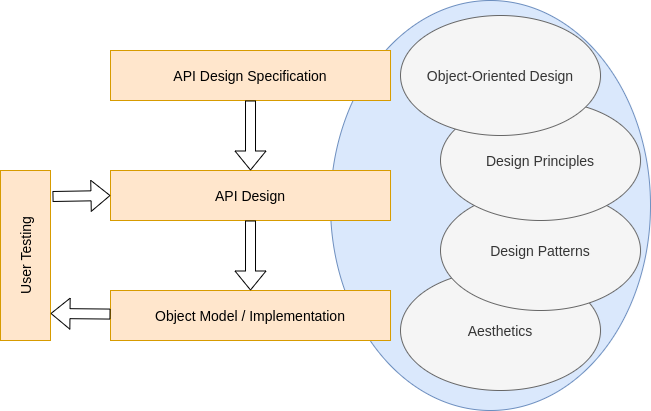
\includegraphics[scale=0.5]{images/api-design-process.png}
        \caption{Api design process}
    \end{figure}

    The API design specification consists a collection of the client-code and scenarios that guide the design of the interface. A scenario is a problem that needs to be solved by the API and the client-code is dream/pseudo code that should solve the problem presented. 

    The design of the interface is the interface’s structure. What areas of the interface can communicate, the file-architecture, which methods are needed and what each class should do. 

    Implementation is the actual code that is written. The details of the implementation should not leak out into the API. Design patterns and principles, and user-testing inform how the physical implementation develops.
    

    \subsection{API Design}

    \subsection{Implementation}

    \subsection{User Testing}

    When we performed the user tests, the method varied a lot each time. Generally call the testers and give them the most updated Jar file and then let them explore the contents first of the framework, and along with it, we would give a set of scenarios for the testers to solve using our framework. At this point we just let them play around with the APIs and get used to it, but most often they would get stuck very fast, and we would have to explain the general gist of the framework and how to use it as intended. Throughout the session we would communicate with them if there were any issues, and if so, we would take notes of the problem.

    After the testers solved the scenarios using our framework, we would have a quick discussion with them about their thoughts and opinions. As they expressed their views on the framework, we would take notes and often ask some follow-up questions. At the end of the session we would ask some general questions to see how their views compared with other testers. This would help us see how the changes affected the framework, as other testers had different opinions.

    After the session with the testers, we would have a discussion with eachother about the feedback we got from the user testing. Since each group member had their own focus areas in the development, this would help a lot to get insight on the next big changes we were going to implement. 

\section{Design Process/Results}

    \subsection{API Design Specification}

        \subsubsection{Builder Pattern}

        We were very quickly guided towards using the Builder pattern when we first had decided on the Framework-type. The Builder pattern, unlike the Abstract Factory pattern, is a lot more like a "Fluent interface", meaning it relies heavily on method cascading.
        The builder pattern is useful as it attempts to seperate the construction of an object from the way it is represented, this way we can use the same process to create many different looking objects that are fundementally similar.

        We needed to use the builder pattern to create immutable objects. We want immutable classes because they have a wide range of benefits when we are developing an API. They are simple to use, they are synchronization safe, we only need one constructor, and they are great for maps(which we're using) to name a few.

        The main problem with implementing the builder pattern is the sheer amount of extra code required. The lines will most likely more than double. However, those extra lines of code give us much more readable code and design flexibility. We exchange parameters in the constructor for much prettier method calls.

        \textbf{Process}

        To develop the API design specification, we employed Scenario-driven design. As a group, we discussed what we wanted this API to do. The requirements that developed from this process needed us to 1: object-orient writing HTML, 2: have an almost one to one translation from HTML-tag to java object, 3: write to file and give that file a .html extension. Based on these three main concepts for the API we created our initial scenarios for how this framework would be used.

        First we need to create a page and we need to be able to populate that page with HTML-elements that can also hold their own internal values like a container of sorts. The objects we put in the container need to be able to have their own functionality written out. This is the basis of what the API needs to be able to do. We need to figure out how the end-user would want to generate their page.
        An example of the first code-iteration:

        \begin{shaded}
            \begin{lstlisting}
                WebPage myPage = new WebPage(); // initialize webpage

                ArrayList<InputField> listOfFields = new ArrayList();
                InputField emailField = new InputField(type: "email", name: "email");
                InputField phoneField = new InputField(type: "phone", name: "phone");
                TextField textField = new TextField(type: "text", name: "text");

                listOfFields.add(emailField);
                listOfFields.add(phoneField);
                listOfFields.add(textField);
                Form myForm = new Form(listOfFields);

                // generates html page in this order
                myPage.generateHeader(); // generate simple header
                myPage.append(myForm);
                myPage.generateFooter(); // generate simple footer
            \end{lstlisting}
        \end{shaded}

        Here we had usage of both high-level and low-level APIs. We could create simple one to one elements and we could automagically generate entire parts of a page.

        Next the user needs to be able to create the body, main, and other semantic containers for their website, but these tags do the same things. Also we need to be able to populate the containers, as well as adding paragraphs and pictures to them.

    \subsection{API Design}

    When designing the APIs in Silhouette, we started writing client-code to see what would work the best. We knew it was important to preserve the advantages of OOP, giving the user control by making objects and manipulating them in various ways. This meant that users have the ability to generate blocks of HTMl quickly with the tools we already know from OOP. We decided to write some client-code to see what would satisfy our requirements, and this would be one of the earliest iterations.

    SHOW CLIENT-CODE HERE
    
    The idea of x was important, and you can see that with the way it's set up and all. But another thing that we couldn't dismiss was the fact that we would get way too many classes if we had kept going the route of making one-to-one relations between classes and HTML tags, following the rule of 30 (Insert Source Here!), so we came up with a secondary solution. Say, for example, the user wants to make a video on their page. The video tag in HTML requires some smaller tags inside it that specifies file and filetypes and controls etc.. an we saw it as an opportunity to hide away these smaller tags within methods. This proved to be a good solution as it both cut down on the total amount of classes, and the user had less things to worry about but still achieve the same things. Eventually we settled on sone one-to-one classes, and some methods to generate simpler HTML code...
    
        \subsubsection{Design Decisions}
        Following best-practices for making APIs, for example, from     

        Later on once we got some feedback from other groups we came across another problem. Users expected to be able to chain multiple methods after eachother. But that was just not possible with how we originally structured our methods and classes, that's where builder pattern comes in. Builder pattern aided the framework in two areas: One, it served as a tool to hide the backend-implementation from the user, and two, it allowed for method-chaining which was exactly what we needed. This mean that previously, the user had to type:

        SHOW CLIENT-CODE HERE

        But now, with the builder-pattern in place, the user can do this:

        SHOW CLIENT-CODE HERE

        However, with Silhouette, we took a different approach using the builder pattern to account for all the different options when writing HTML and CSS. The pattern creates a structure in the code that consists of building components and appending them to each other. With Spring, the user builds a component through the factory pattern that initalizes the beans by following given instructions, but we thought the builder pattern would be more flexible on the go:

        \begin{shaded}
            Creating a paragraph and adding it to a div
            \begin{lstlisting}
                Paragraph p = new Paragraph.Builder()
                        .setText("Hello World")
                        .build();
                Container div = new Container.Builder()
                        .addElements(p)
                        .build();
            \end{lstlisting}
        \end{shaded}

        \subsubsection{Personal Decisions}
    
        \subsection{Implementation}

        Implementation was done in various stages as we had many ideas for how we wanted the resulting framework to behave. After a lot of discussion with the group, we began writing client-code to help us visualize the API to get better ideas on how we got incorperate the implementation. After several supervisions with the lectruer, we were advised to us a builder-pattern, which works wonders for the type of tasks we want to do, however it makes implementing a bit of a chore, as this means usually our source-code will double. Getting to understand how this pattern works was not easy, since as we were writing our API-code we did not have a full understanding of the structure of method-calls/chaining, nor how to really instantiate these objects. This led to some early errors like giving each builder-class a specific name, and not implementing it correctly.
    
        After getting to understand these things there are other issues that appear throughout. We have some global attributes that all objects in the API share, so it's logical to just write the method once and be done with it, however this does mean that casting between classes becomes necessary. This is possibly because we opted for internal static Builder classes. We felt that was the most logical and direct connection we could make between an objects and its builder.
    
        Lastly, we needed to form a system to generate the actual. The big idea was to make some sort of compiler that puts strings together to make the necessary web files. It later became apparent that we needed one compiler for each API, as the logic and syntax are wastly different. As it stands, the compilers will either read html and css in the form of Strings, or plain java old objects (POJOs). Then once the user is done defining their pages and stylings, they will inform the respective compiler to perform a compile and generate the web files. If these files already exist, the compiler should just overwrite them to apply the new changes.


    \subsection{User Testing}

    User testing started after a month of developing the first iteration of the API. At this point the low-level HTML API felt almost complete, however the high-level-, and CSS-APIs were bare minimum. The implementation was not ready and the APIs consisted of plain old java objects. It was therefore important know if the names and overall use made sense, and if there were any major flaws that we could improve upon.


    (THIS NEEDS TO BE CHANGED)
    right after all the classes that was needed to build am HTML document and the same for the CSS part. At this time the code was just object oriented programming and it flet easy to use, but it was alot of unnecessary writing and to a degree hard to follow.   
        
    After the first user testing with another group, we didn't get alot of crtical feedback on whats "good" and "bad" excepted for the things that we knew about, but we got feedback on the logical structure part and that is one of the things we needed.
        
    After some time we knew what we wanted the code ot looke like and how to simplify it more, and that is when we started to use "Builder pattern" instead of the heavy object coding we had previously. This made it more readable for the eyes and work with.

        \subsubsection{Frist user testing session (Silhouette-HTML v.2)}

        Right after they had tested our framework and completed the setup, we asked them to give their initial reaction and opinion. They said, “It was pretty good once we got the hang of the class names” which was a relief to hear. It seemed to us that they found the APIs to be intuitive, as they quickly grew familiar with the main classes. We then followed up with a few questions regarding their experience, and they told us they could easily expand further on their website with enough practice.

        \subsubsection{Second user testing session (Silhouette-HTML v.2)}

        This user testing toke more time that what was needed, if it wasn’t for an error from our side in the code structure. When we found out what the error was and the confusion was over, it was back to the user testing, but the person that was testing the program was stuck and didn’t understand how to start and/or what to write (defining the html-object). After some time we gave the user a push in the right and the user started to type/write like it was natural for them or as the hade used our framework before.

        \subsubsection{Third user testing session (Silhouette-HTML v.2)}

        In this user testing the tester was tested in a different way, where the tester received minimal help and mostly through think and some fiddling on their own, because of the users higher understating to code structure and language.

        The user managed the first part of the task easily (due to the naming of classes and method names) but began to strive on the second task. The user was supposed to create a new object called "Container", but started working on the method calls instead (because it seemed most natural to them) and had to ask for help and then came the next problem... what are Builders.

        After some explanation it came naturally and the rest of the second task was then over and the user was on their owe, with a little hint here and there. The user could see the logic but felt that it lacked a flow in the structure and believed that getting in to "Silhouette" for a new user is not easy without a manual or help from someone.
        
        \subsubsection{Fourth user testing session (Silhouette-HTML v.3)}

        Fourth testing was done in a group context, where one of them wrote and the others watched and tried to understand "Silhouette" (I also had to describe how Builders works).

        It started the same with this group as it was done with the other user testing section, but since one of the user was looking through the library and was reading the methods that had a similar name as in HTML, one tester got an idea what to write and they managed to complete this task. And they applied the same tactic to the next tasks, and they managed the whole user testing with a few hints. 

        \subsubsection{Fifth user testing session (Silhouette-HTML v.3)}

        The fifth test was carried out by a student with a good knowledge of java and HTML, who wanted to learn the framework (“Silhouette”) from top to bottom. The user spent 1 hour and 30 min doing the task (without help) and gained insight into how "Silhouette" HTML.BaseComponents.* (file's) worked. This user was more interested in the "Silhouette" library and gave some feedback about that the structure is easy to understand, but there was a lack of comment (you can read comments for a jar file) on what the methods do/did, etc. and that the end result might affect a user “Silhouette’s code” and meant that “it’s too hard-coded” when a user is done with it.

        \subsubsection{Last user test}

        For the last user test we tested with a student who previously had the same framework course, and who was very familiar with builder pattern and API design. The session took about three hours, and we tested both the HTML API and the CSS API. We sent him the Jar file of the newest version of the framework, a type reference documentation, and some scenarios to solve with the framework.

        \textbf{Make a new HTML page. Set a custom title, and set the charset meta tag to "UTF-8"}

        \textbf{Scenario 17}

        For scenario 2, the user were instructed to make a body element and add it to the page. At first, it wasn't very obvious form him to use the Container object to build the body element, as it is passed through the parameter. After some explanation, he understood why we had done it that way, but still felt like it was not as intuitive. He commented that it would be much better to just separate the most important layout elements into their own class, though this was already discussed within the group at the beginning of the project. Having a class for each element comes with two major issues. Firstly, if we would simply make a class for each element, there would be too many classes to keep track of. Secondly, how would we decide which element needed their own class? Because of this we decided to keep it as originally planned.

        \textbf{Scenario 18}

        Here he found it confusing that there were two ways of adding a heading to a container element. While the intended solution was to make a Heading object, he opted for the addHeading method inside ContainerElement.

        \begin{shaded}
            Making a Heading object

            \begin{lstlisting}
                Heading myHeading = new Heading.Builder()
                        .setLevel("h1")
                        .setText("My heading")
                        .build();
            \end{lstlisting}

            Using the addHeading method inside ContainerElement

            \begin{lstlisting}
                Container div = new Container.Builder()
                        .addHeading(1, "My heading")
                        .build();
            \end{lstlisting}
        \end{shaded}

        Initially, this was done to give users more options when declaring the markup. However, this proved to be more confusing then helpful, so we decided to remove this additional method.

        \textbf{Scenario 19}

        Right off the bat, his impression was that we had over-used the builder pattern, to the point where it becomes unecessarily complicated. For example, he explained how it was unecessary to use builder pattern for the Paragraph class, as the paragraph should only take one argument in the constructor anyway. He suggested that it would be better to simply pass the text to the constructor.

        \begin{shaded}
            With builder pattern

            \begin{lstlisting}
                Paragraph p = new Paragraph.Builder()
                        .setText("Hello, World!")
                        .build();
            \end{lstlisting}

            His suggestion

            \begin{lstlisting}
                Paragraph p = new Paragraph("Hello, World!");
            \end{lstlisting}
        \end{shaded}

        His suggestion was not bad, but since we wanted to follow the same convention for every class, we felt it was better to leave it as be with the builder pattern. That way, there is not confusion whether it uses the builder or not. We also find the parameters more clearer with builder pattern, as it explicitly shows it in the method name.

        \textbf{Scenario 20}
        
        At first he was not fond of using enums when adding a new rule to the rule set, but quickly he grew the habit of using them. He commented that it felt unecessary at first, and that he would rather type in the propeties and values as a string. But after explaining why we use them (which is to make sure the user does not pass inn misspellings), he understood and agreed that it was a good solution.

        \textbf{Scenario 21}

        
                

        To finish off the session, we asked him some general questions about the framwork. Firslty, we asked him about what he thought about the name "Silhouette", and if he found it intruiging and informative. To this, he told us that the name is as ambiguous as most other names out there. He stressed, that it does not necessarily mean it is bad, but it did not give him any idea of what the framework did. At this point, we have become very fond of the name, but it is always nice to get feedback.

        We also asked him if he found the framework to be difficult to use. To this he responded that builder pattern greatly increases the amount of code needed to generate a website, so in this case it would be faster to write it in standard HTML and CSS. We agree to this, wowever, we are still of the belief that the OOP aspects and the additional make up for it. Another issue for him was the quality of the type reference documentation, as it often failed to give him a good idea of what each class represented.

\section{Resulting Framework}

\section{Discussion}

The plan is to make a html-structure in Java by using object-oriented code structure.

In the first phase we were working together all the time. We collected as much information that we could find, about html and css. And after some working sessions we had a 1 to 1 structure (of the Java-code to html and css part). The css part was straightforward when it came to the structure part, but the problem was in the html. We found new and better ways all time to make the client code easier and more understandable.

In the second phase we have agreed that this is what we need for “Silhouette” to be able to create web pages. At this point we are working on the html part and hope that we can start on user testing aright away. After some user testing, we start on the third phase and now that we knew what we want the code structure to look like, we start to specializing us (and you can se that in the “Delegation of work”). 

\section{References}
[1]:  Chevalier-Boisvert, M. (2015). \textit{The Problem with HTML}. \\ Retrieved from https://pointersgonewild.com/2015/04/16/the-problem-with-html/

\end{document}